\section{Simulation results}
The simulation was performed in Sinalgo\footnote{http://www.disco.ethz.ch/projects/sinalgo/}.
Sinalgo is a simulation framework which can test and validate network algorithms and at the same time it offers a graphical view on the programmed processes as well as a fast batch mode.

There are two different simulation runs.
The first one calculated the Euclidean and hop spanning ratio of PDT and RMYS and the second one counted the messages which were needed to construct PDT, RMYS and the amount of messages needed by two hop beaconing.
Both simulations had 1000 random connected graphs for each node density, which went from 5 to 20.
The numbers of nodes $n $ used for each density were calculated with the following formula:
\begin{equation*}
n =round( \frac{D_x \cdot D_y}{\pi \cdot R^2} \cdot density)
\end{equation*}
Hereby, $D_x=1000 $ and $D_y=1000 $ are the dimension of the simulation plane and $R = 100 $ is the unit disk radius.

\bigskip

The simulations are based on the following assumptions.
\begin{itemize}
\item All nodes are static meaning they cannot move.
\item All calculations are ordered into synchronous rounds. 
At the beginning a node receives all messages sent in the round before.
It follows a general calculation phase and at last a node can send messages.
\item Messages arrive instantaneously and cannot get lost.
Every message which was sent, arrives for sure in the round after it was sent.
\item There are no 4 nodes which are co-circular.
\item All graphs are connected.
\end{itemize}


Figure \ref{fig:RMYS_PDT_SpanningRatio} shows the measured spanning ratio of RMYS and PDT to the unit disk graph with respect to node density.
It is noticeable that both lines seem to be the same line.
For density $5 $ the ratio is approximately $1.30 $ and density 20 has approximately a spanning ratio of $1.38 $.
In between 5 and 20 the curve is increasing slightly and has no outliers.

Since both lines are almost identical it is possibly true that RMYS has also a constant spanning ratio which is a fractional amount greater than the proven spanning ratio of PDT (refer to \cite{Neumann2012} for proof), which is smaller or equal to $\frac{1+\sqrt(5)}{4} \pi^2 $. 

\begin{figure}[h!]
\centering
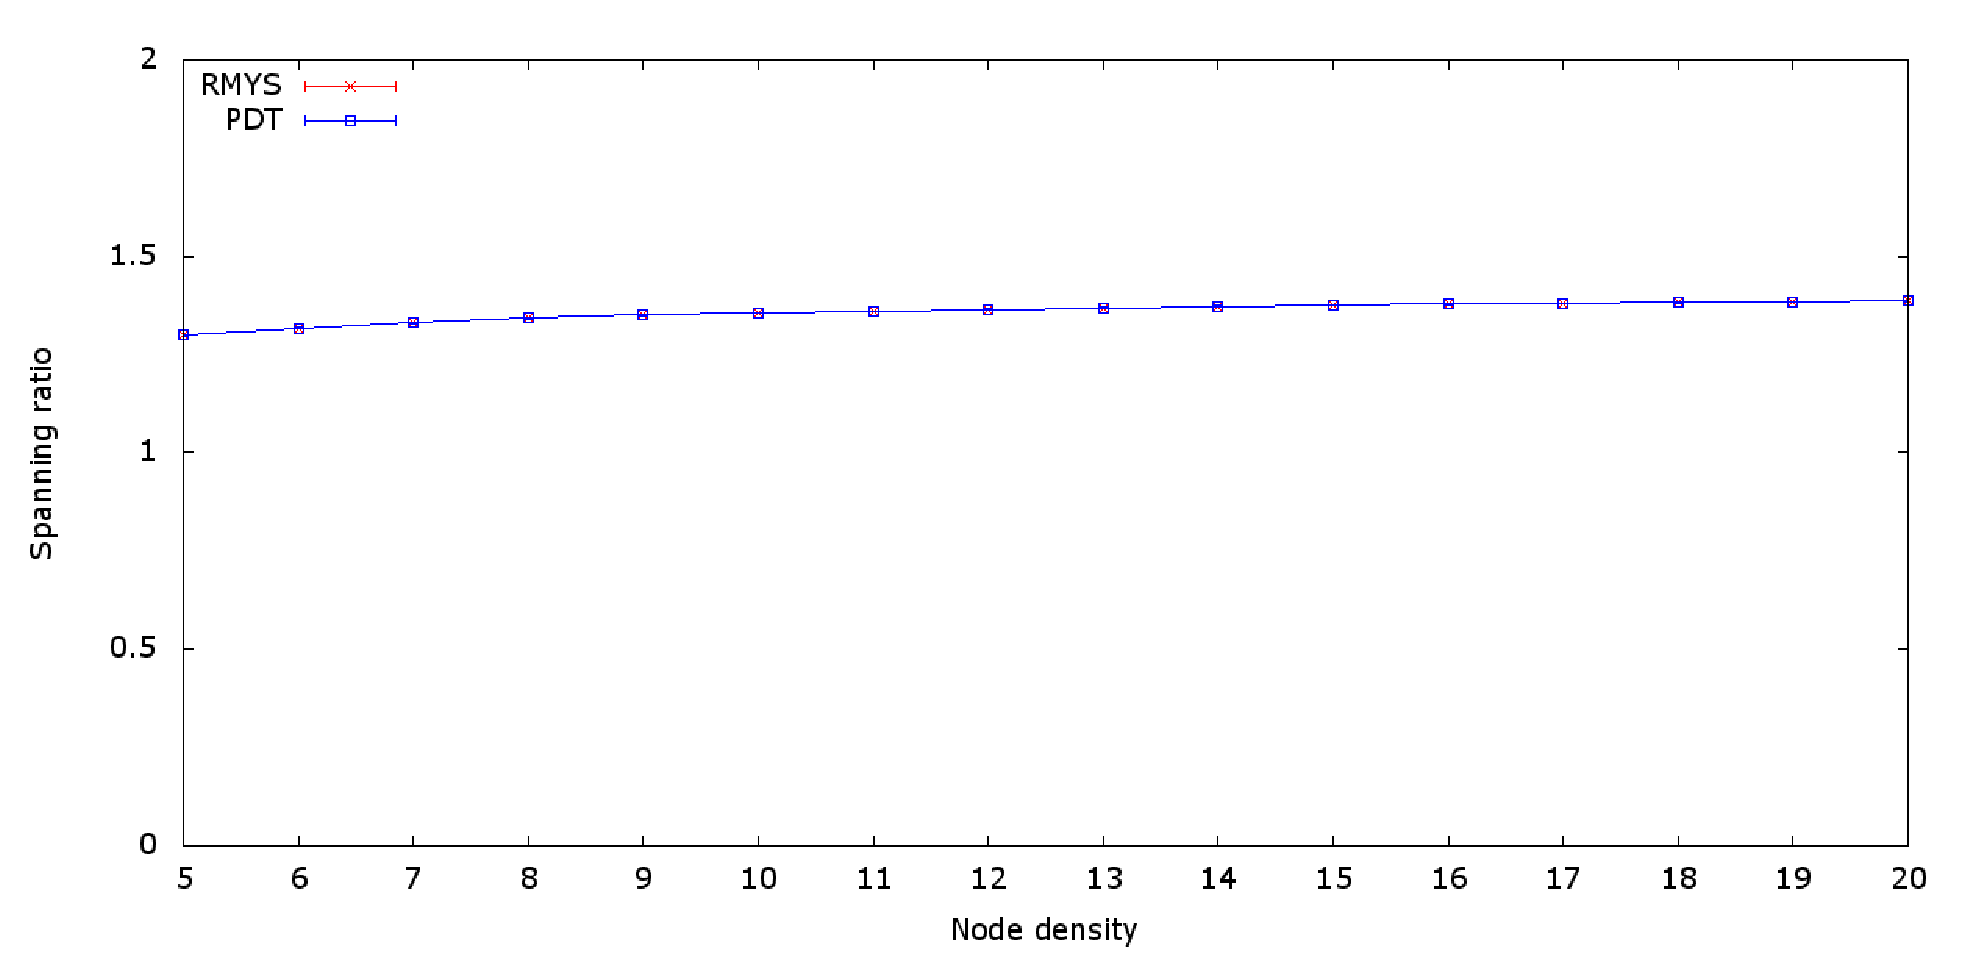
\includegraphics[width=1.2\linewidth]{eps/RMYS_PDT_SpanningRatio.eps}
\caption{Euclidean spanning ratio of Reactive Modified Yao Step (RMYS) and Partial Delaunay Triangulation (PDT) with respect to the Unit Disk Graph in context to the node density. 1000 Simulations per density.}
\label{fig:RMYS_PDT_SpanningRatio}
\end{figure}


Figure \ref{fig:RMYS_PDT_HopSpanningRatio} shows the measured spanning ratio of RMYS and PDT to the unit disk graph with respect to node density.


\begin{figure}[h!]
\centering
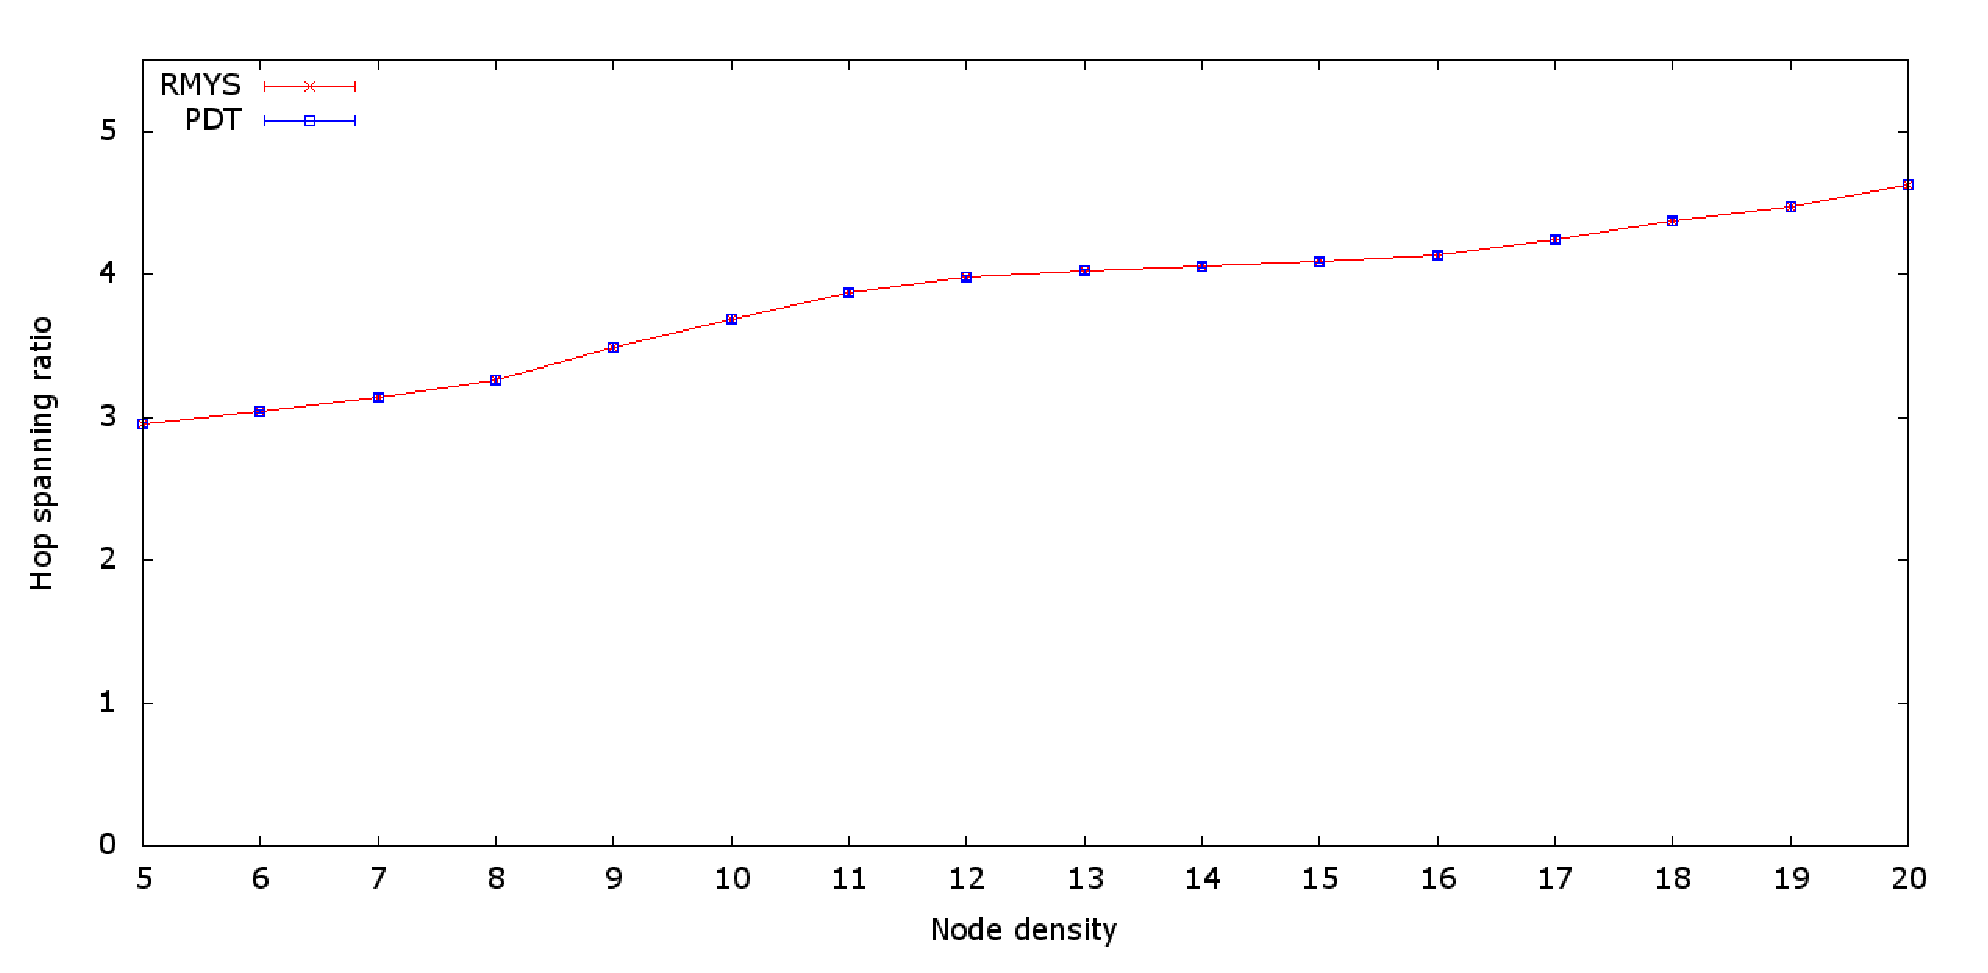
\includegraphics[width=1.2\linewidth]{eps/RMYS_PDT_HopSpanningRatio.eps}
\caption{}
\label{fig:RMYS_PDT_HopSpanningRatio}
\end{figure}




%While calculating the spanning ratios of both graphs a global algorithm was used, which granted every node knowledge about the complete graph.



